\documentclass[12pt]{article}%
\usepackage{amsfonts}
\usepackage{fancyhdr}
\usepackage[hidelinks]{hyperref}
\usepackage[a4paper, top=2.5cm, bottom=2.5cm, left=2.2cm, right=2.2cm]%
{geometry}
\usepackage{times}
\usepackage{caption}
\usepackage{subcaption}
\usepackage{amsmath}
\usepackage{nccmath}
\usepackage{listings,newtxtt}
\usepackage{changepage}
\usepackage{amssymb}
\usepackage[titletoc]{appendix}
\usepackage{biblatex}
\usepackage{hyperref}
\usepackage{graphicx}%
\usepackage{float}
\usepackage[nottoc,numbib]{tocbibind}
\addbibresource{references.bib}
\settocbibname{References}
\setcounter{MaxMatrixCols}{30}
\newtheorem{theorem}{Theorem}
\newtheorem{corollary}[theorem]{Corollary}
\newtheorem{definition}[theorem]{Definition}
\newtheorem{lemma}[theorem]{Lemma}
\newtheorem{proposition}[theorem]{Proposition}
\newenvironment{proof}[1][Proof]{\textbf{#1.} }{\ \rule{0.5em}{0.5em}}

\begin{document}
\title{NBA Team and Player Rankings using Networks\\
\vspace{3 mm}
\large ELE/COS 381 Interim Report}
\author{Daniel Chae \& Drey Tengan}
\date{\today}
\maketitle

\tableofcontents
\newpage
\section{Introduction and Problem Statement}
\subsection{Introduction and Background}
\null\quad\quad In class, we learned about the PageRank algorithm \cite{PageRank} that allows search engines like Google to efficiently navigate a complex network of webpages based on importance scores. Stemming from our common interest in sports, we were drawn to the idea of applying the PageRank algorithm to sports, specifically to the National Basketball Association (NBA).\\
\null\quad\quad Currently, there exist many metrics that analyze the performance of teams, one primary metric being their win-loss records. Furthermore, there are numerous analysts attempting to predict the outcome of future NBA games and the NBA Playoffs. However, very few of these efforts involve complex networks - most rely on quantiative and qualitative features of teams (e.g. team X has player Y, who has excelled in offense and defense). In fact, in the NBA Power Rankings website, there is a statement: ``NBA.com's Power Rankings, released every Monday during the season, are just one man's opinion. If you have an issue with the rankings, or have a question or comment for John Schuhmann, send him an e-mail or contact him via Twitter'' \cite{nbapowerrating}. This statement indicates that there is some fundamental human-level bias that cannot be waived away. Given the potential of the vast amount of performance data available, more reliable, systematic predictions can be made using the PageRank algorithm or variations on the algorithm.\\
\null\quad\quad Vincent Xia and Kavirath Jain, students of a previous semester of ELE 381, used the PageRank algorithm to predict outcomes of games and rankings of teams in the National Football League (NFL) and the National Basketball Association (NBA) \cite{XJ}. They compared performance of teams and created a predictive ranking of teams using two methods: baseline and weighted. While their procedure yielded about 0.6-0.65 accuracy rate for NFL games, it was less predictive for NBA games. In his 2012 book \textit{The Success Equation}, Michael J. Mauboussin \cite{nbapredictable} claims that of the five major U.S. sports, basketball is the easiest to predict and the most dependent on skill rather than luck, with American football being the ``luckiest'' sport besides hockey. This indicates that there is room to improve analysis and prediction for teams in the NBA, considering that the $0.6-0.65$ accuracy range is just above $0.5$ accuracy, which is just as good as just randomly guessing outcomes.
\subsection{Problem Statement}
\label{sec:1.2}
\null\quad\quad We use network structures, algorithms, and data to better predict the outcome of NBA games. Xia and Jain's weighted method (an adaptation from Govan et al. 2008 \cite{Govan}) is used as a control and we offer three new alternative ranking methods: Average Point Differential (APD), Deviant Baseline (DB), and Pick on Someone Your own Size (PSYS). All of these methods are further detailed in Section \ref{sec:2} of this report. After models are trained, we use a test set to study the accuracies of the models.\\
\null\quad\quad Another main component of this study is player analysis. Xia and Jain focused on the performance and ranking of teams as a whole. We expand the analysis to consider specific players and their performance against players from other teams. This is an effort that has not been algorithmically attempted. We break this down into two major components: team-pair and All-Star. For team-pair analysis, we select two teams and create networks amongst the players of the two teams using their offensive ratings (ORtg), defensive ratings (DRtg), and their box plus minus (+/-). The goal is to determine the set of players on both teams that would maximize their own team's performance in the game. For All-Star analysis, we create a network on +/-. The network seeks to rank all players in the NBA to determine the best player in the league, best players for each time, and the best players on the Eastern and Western Conferences. We compare the two different networks that each generate their own ranking list of the players. These components are further discussed in Section \ref{sec:2}.

\section{Dataset and Networks}
\label{sec:2}
\subsection{Dataset and Scraping Data}
\null\quad\quad Data was obtained from \href{https://www.basketball-reference.com/}{Basketball-Reference.com}, a site that condenses official NBA stats (verified with official stats available from ESPN.com) in a way that is more conducive for the scraping algorithm. We focus on the 30 NBA teams and all 540 players in the 2018-19 season. As mentioned in the Problem Statement, (Section \ref{sec:1.2}) the study analyzes two major sets of networks. One set of networks looks to study team performances against other teams. The goal was to generate a ranking of the teams. This is further explored in Section \ref{sec:2.2}. The second set of networks looks to study individual players against players from other teams, further discussed in Section \ref{sec:2.3}. \\
\null\quad\quad The data was scraped using the BeautifulSoup Python package, stored in pandas DataFrames, manipulated on NumPy, and saved as csv files. The preliminary work for this report includes the analysis using weighted method, APD, and DB for team rankings. See the Appendix A for the Python code for scraping, manipulating, and running the PageRank using the three methods.
\subsection{Team Ranking Networks}
\label{sec:2.2}
\null\quad\quad First, team networks were created to compare the performance of teams as a whole and determine the rankings of teams using different methods. Each of four methods was used to create a network matrix $A$, which is then row-normalized to yield \textbf{H}, which is then used to generate importance scores, $\pi_i$, for each of the methods numbered $i=\{1,2,3,4\}$, using the PageRank algorithm. For the sake of illustrating the four methods, suppose there are only three teams, Golden State Warriors (GSW), Houston Rockets (HOU), and Minnesota Timberwolves (MIN), with match outcomes specified in Table 1.
\begin{center}
\captionof{table}{An example set of matches for the three teams}
\begin{tabular}{|c|c|c|c|}
\hline
\textbf{Team 1} & \textbf{Team 2} & \textbf{Score} & \textbf{Winner}\\
\hline
Warriors & Rockets & 86-107 & Rockets\\
Rockets & Timberwolves & 91-103 & Timberwolves\\
Warriors & Rockets & 104-106 & Warriors\\
Warriors & Timberwolves & 116-99 & Warriors\\
Rockets & Timberwolves & 111-121 & Timberwolves\\
\hline
\end{tabular}
\end{center}
\begin{enumerate}
\item \textbf{Weighted Method}\\
  \null\quad\quad The weighted method is the same weighted method used by Xia and Jain \cite{XJ}. It was employed for the analysis as a control. Suppose there is a square matrix $A$ and let $A_{}[i,j]$ denote the entry of team $i$ against team $j$, where $i$ denotes rows and $j$ denotes columns. Then each of the entries are
  \[
  A_{1}[i,j]=
  \begin{cases}
  \sum_{N_{i\rightarrow j}}d_{ij} &\text{ $i$ lost to $j$}\\
  0 &\text{ otherwise}
  \end{cases}
  \]
  Each of the entries $(i,j)$ is a sum of the point differentials, $d_{ij}$, of the $N$ games where team $i$ lost to team $j$. Using the example setup indicated in Table 1, we have the network shown in Figure 1 and the network matrix $A_1$, which is row-normalized to get $\textbf{H}_1$.
  \begin{figure}[H]
	\centering
	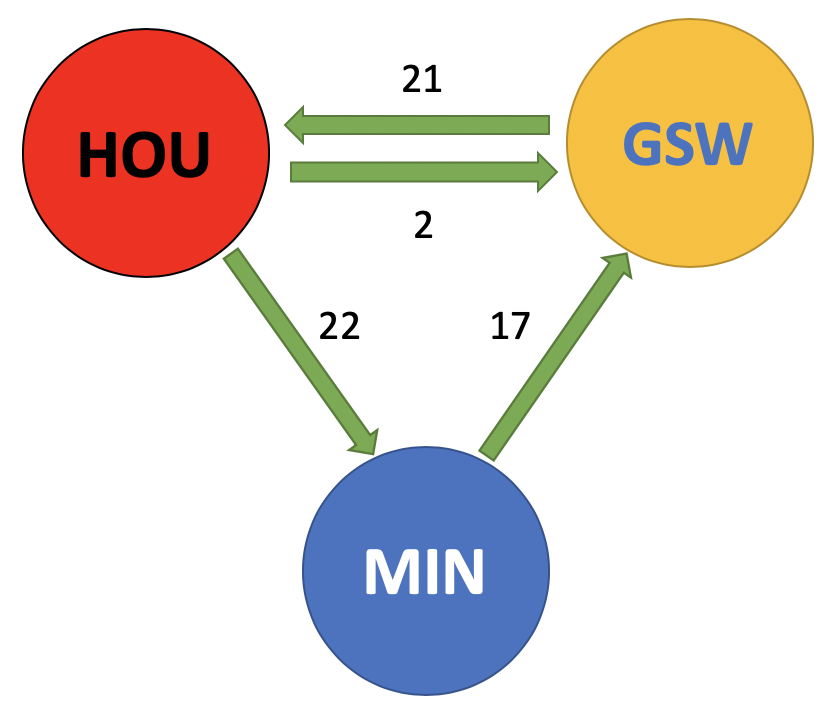
\includegraphics[width=2in]{./images/weighted.png}
	\caption[Network using the Weighted Method]{Network using the Weighted Method}
\end{figure}
\begin{align*}
A_1 =\begin{bmatrix}0 & 21 & 0\\2 & 0 & 22\\17 & 0 & 0\end{bmatrix}, \textbf H_1=\begin{bmatrix}0 & 1 & 0\\0.0833 & 0 & 0.9167\\1 & 0 & 0\end{bmatrix}
\end{align*}

  \item \textbf{Average Point Differential (APD)}\\
  \null\quad\quad The APD method is taking the entries in the weighted method and dividing it by the number of games associated with the entries. This is shown by 
  \[
  A_{2}[i,j]=
  \begin{cases}
  \frac{\sum_{N_{i\rightarrow j}}w_{ij,N}}N &\text{ $i$ lost to $j$}\\
  0 &\text{ otherwise}
  \end{cases}
  \]
  Using the example setup, we get the network shown in Figure 2. The motivation behind using this method is to generate directed edges that would scale down deviant blowout games. Meaning, if team $A$ beat team $B$ 5 times with point differential $d_{BA}=\{3,5,2,4,21\}$, the last game with differential $21$ will be scaled down so that the performance of $B$ against $A$ is better indicated with the average of $7$. We take the average instead of the median because we want to leverage the sensitivity of the average to outliers - we still want to indicate that there have been blowout games while still indicating ``average'' performance. 
  \begin{figure}[H]
	\centering
	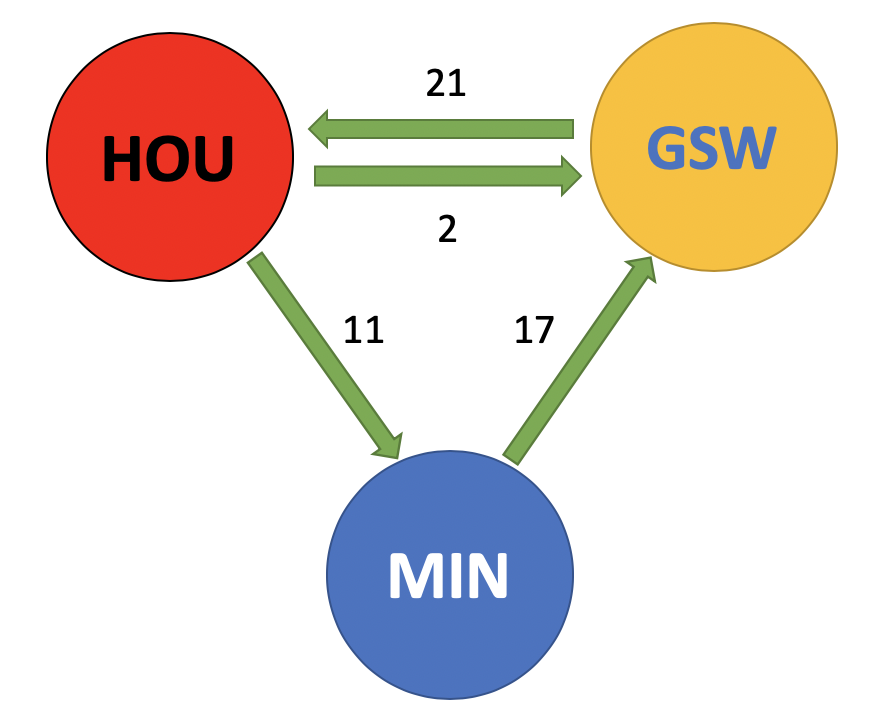
\includegraphics[width=2in]{./images/APD.png}
	\caption[Network using the APD Method]{Network using the APD Method}
\end{figure}
\begin{align*}
A_2 =\begin{bmatrix}0 & 21 & 0\\2 & 0 & 11\\17 & 0 & 0\end{bmatrix}, \textbf H_2=\begin{bmatrix}0 & 1 & 0\\0.1538 & 0 & 0.8462\\1 & 0 & 0\end{bmatrix}
\end{align*}
  
  \item \textbf{Deviant Baseline (DB)}\\
  \null\quad\quad The DB method is a deviation from Xia and Jain's baseline method, where the directed edge is a binary indicator between teams. For entry $A_{}[i,j]$, the value is $1$ if team $j$ beat team $i$ at some point in the history of all games and $0$ otherwise. Intuitively, this is a weak network because stronger teams that repeatedly beat weaker teams should be rewarded. Therefore, we propose the DB method, which uses the total number of wins of team $j$ over team $i$. Formally,
  \[
  A_{3}[i,j]=
  \begin{cases}
  \sum_{N_{i\rightarrow j}}1 &\text{ $i$ lost to $j$}\\
  0 &\text{ otherwise}
  \end{cases}
  \]
  This produces the network shown in Figure 3. Notice that in this method, the point differential does not matter. The only consideration is the number of victory itself.
  \begin{figure}[H]
	\centering
	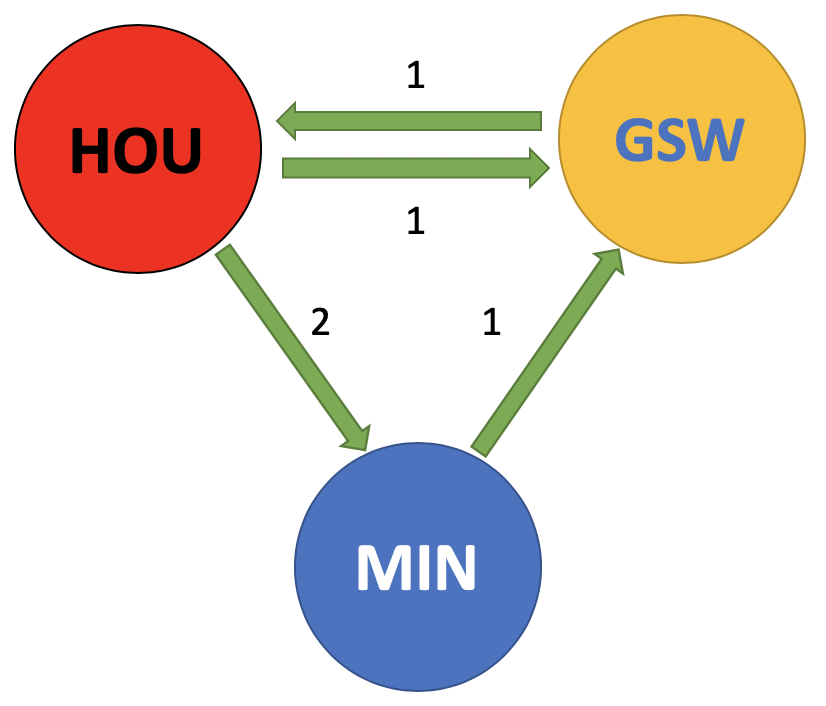
\includegraphics[width=2in]{./images/DB.png}
	\caption[Network using the DB Method]{Network using the DB Method}
\end{figure}
\begin{align*}
A_3 =\begin{bmatrix}0 & 1 & 0\\1 & 0 & 2\\1 & 0 & 0\end{bmatrix}, \textbf H_3=\begin{bmatrix}0 & 1 & 0\\0.333 & 0 & 0.667\\1 & 0 & 0\end{bmatrix}
\end{align*}

  \item \textbf{Pick on Someone Your own Size (PSYS)}\\
  \null\quad\quad Suppose now that there is a pre-ranking of the teams, determined by their win-loss record. PSYS method creates a network which greatly rewards wins of low-rank teams over high-rank teams and rewards lightly on wins of high-rank teams over low-rank teams. The intuition here is such that a highly ranked team will not benefit from continually defeating poorly performing teams. Formally, suppose that there is a rank vector $\textbf{r}$, $r_a$ is the rank of team $a$, and there are $T$ total teams. If $r_i > r_j$, then team $i$ is ranked lower than rank $j$, vice versa. Then each of the entries are
  \[
  A_{4}[i,j]=
  \begin{cases}
  \Big(1-\Big(\frac{r_i-r_j}{T}\Big)^2\Big)\sum_{N_{i\rightarrow j}}1 &\text{ $i$ lost to $j$, }r_i > r_j\\
  \Big(1+\Big(\frac{r_i-r_j}{T}\Big)^2\Big)\sum_{N_{i\rightarrow j}}1 &\text{ $i$ lost to $j$, }r_i < r_j\\
  0 &\text{ otherwise}
  \end{cases}
  \]
  The first term in the first two cases of the piecewise, $\Big(1-\Big(\frac{r_i-r_j}{T}\Big)^2\Big)$ for $r_i > r_j$ and $\Big(1+\Big(\frac{r_i-r_j}{T}\Big)^2\Big)$ for $r_i < r_j$, is called the rank factor, $f_r$. Notice how in this case, we use the number of wins, rather than point differential. If we use point differential, then we would just sum up the total point differentials, $d_{ij}$, much like in the Weighted Case (Section 2.2.1), and apply the rank factor. For this project, we use both methods of PSYS. PSYS-1 is used to denote the method using the number of wins (as shown above) and PSYS-2 is used to denote the method using point differentials.\\
  \null\quad\quad Given the example, the win loss records of each of the teams are: Golden State Warriors have a record of $2-1$, Houston Rockets have a record of $1-3$, and Minnesota Timberwolves have a record of $2-1$. Since the Timberwolves lost to the Warriors, the ranking becomes: Warriors are 1st, Timberwolves are 2nd, and Rockets are 3rd. This means that $\textbf{r}=(1,3,2)$. We run through the PSYS-1 calculation for Timberwolves versus Rockets as an example:\\
  \null\quad\quad Since the Timberwolves never lost to the Rockets, we only consider the matrix entry $A_4[1,2]$ (recall that the matrix entry is zero-indexed, team $0$ being Warriors, team $1$ being Rockets, and team $2$ being Timberwolves). Since the Rockets are ranked lower, meaning $r_1>r_2$, the first case applies. The rank factor $f_r=1-(\frac{1}{3})^2=\frac{8}{9}$. Since there are two wins, the entry $A_4[1,2]=\frac{16}{9}\approx 1.778$. We extend this for all matrix entries and for PSYS-2 to get the following networks (Figure 4) and matrices:
  \begin{figure}[H]
  \centering
\begin{subfigure}{.5\textwidth}
  \centering
  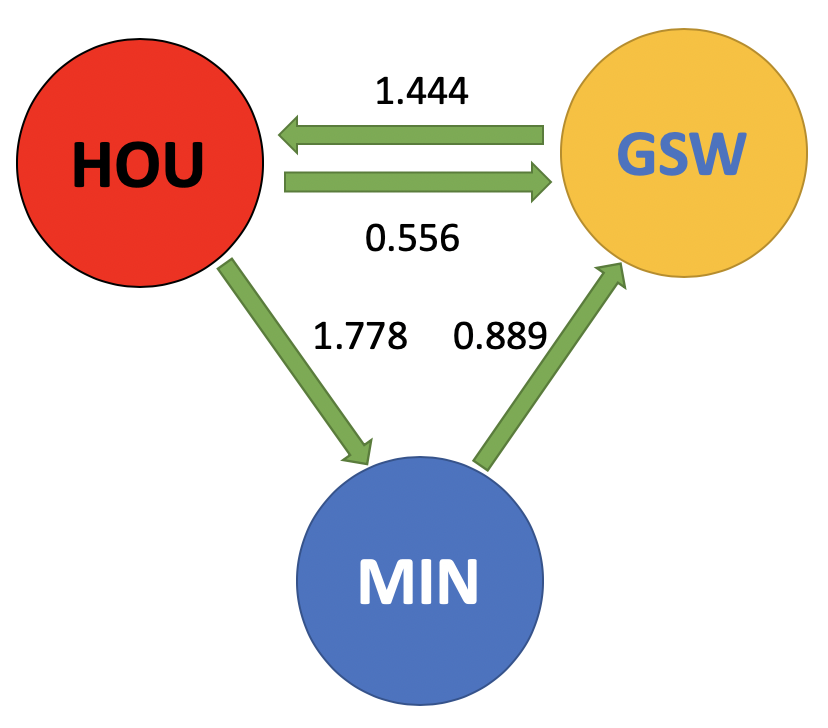
\includegraphics[width=2in]{./images/PSYS-1.png}
  \caption{Network using PSYS-1}
  \label{fig:sub1}
\end{subfigure}%
\begin{subfigure}{.5\textwidth}
  \centering
  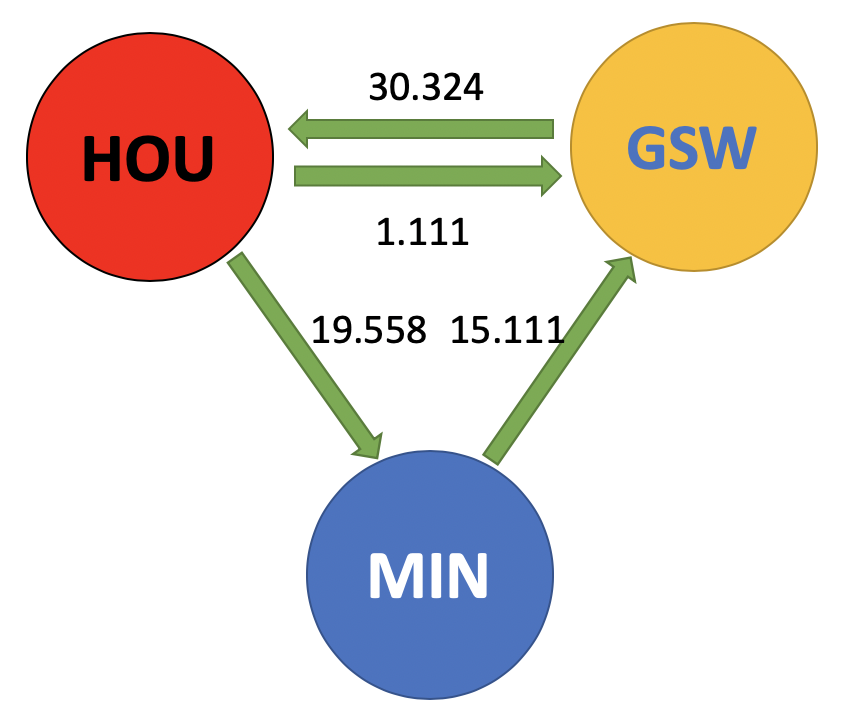
\includegraphics[width=2in]{./images/PSYS-2.png}
  \caption{Network using PSYS-2}
  \label{fig:sub2}
\end{subfigure}
\caption{Networks created using PSYS method}
\label{fig:test}
  \end{figure}
  \begin{align*}
&A_{4,1} =\begin{bmatrix}0 & 1.444 & 0\\0.556 & 0 & 1.778\\0.889 & 0 & 0\end{bmatrix}, \textbf H_{4,1}=\begin{bmatrix}0 & 1 & 0\\0.238 & 0 & 0.762\\1 & 0 & 0\end{bmatrix}\\
&A_{4,2} =\begin{bmatrix}0 & 30.324 & 0\\1.111 & 0 & 19.558\\15.111 & 0 & 0\end{bmatrix}, \textbf H_{4,2}=\begin{bmatrix}0 & 1 & 0\\0.054 & 0 & 0.946\\1 & 0 & 0\end{bmatrix}
\end{align*}

\end{enumerate}
\subsection{Player Ranking Networks}
\null\quad\quad A player's performances against other players was studied using networks and the PageRank algorithm. The analysis for player ranking is further divided into team-pair analysis (Section 2.3.1) and All-Star analysis (Section 2.3.2). Both of these networks determine the ranking of players, but team-pair focuses on player performance against specific teams and All-Star generalizes for all players in the NBA.
\subsubsection{Team-pair Analysis}
\null\quad\quad While there are prior studies on team performances using networks, there are very limited studies on player performance using networks. Player performance was studied by pairing teams together and analyzing player metrics for the specific team. Each node is a player and directed edges will be based on box plus minus (+/-). For the preliminary analysis, we actually used the difference between offensive rating (oRtg) of players and defensive rating (dRtg) of opposing players. We discovered that there are actually problems with structuring a network in this way, further discussed in Section 3. Moving forward, we intend to focus on the +/- metric. Suppose the +/- of player $i$ is $m_i$. Then a matrix where entries indicate directed edges in a network can be constructed.
  \begin{align*}
  f(m,v)&=\begin{cases}
  m^2\cdot v\quad\quad \text{if }m>0.25,\text{ at least 1 game}\\
  -10\quad\quad\quad\text{otherwise}
  \end{cases}\\
  A[i,j]&=
  \begin{cases}
  x=f(m_j,v_{j,A})-f(m_i, v_{i,B}) &\text{if }x>0\\
  0 &\text{otherwise}
  \end{cases}
  \end{align*}
As an example, suppose there are two teams, $X$ and $Y$ with two players each, indexed $i\in\{1,2\}$. Table 2 has the +/- of the four players.
\begin{center}
\captionof{table}{Example +/- values for two teams, each with two players}
\begin{tabular}{|c|c c c c|}
\hline
\textbf{Players} & $X_1$ & $X_2$ & $Y_1$ & $Y_2$\\
\hline
\textbf{+/-} & 10.1 & -5.6 & 3.7 & 12.2 \\
\hline
\end{tabular}
\end{center}
This results in the network shown in Figure 5. Note that the matrix is in the order of $X_1,X_2,Y_1,Y_2$ row-wise and column-wise. Since there are 30 NBA teams, 435 network pairings are studied.
  \begin{figure}[H]
	\centering
	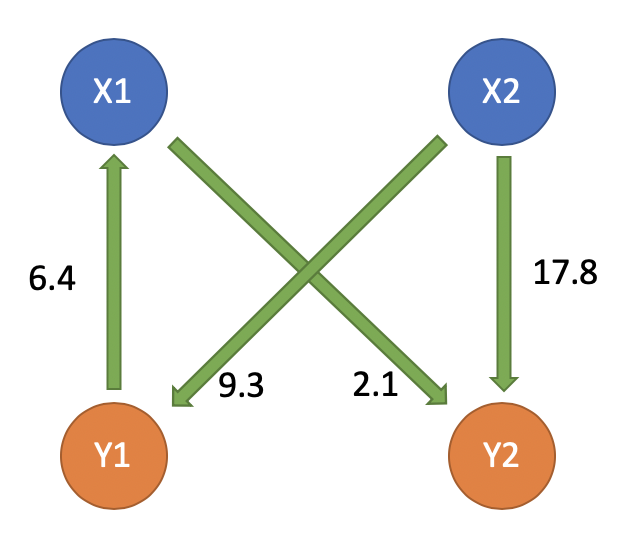
\includegraphics[width=2in]{./images/team.png}
	\caption[Network for team-pair analysis of +/-]{Network for team-pair analysis of +/-}
\end{figure}
\begin{align*}
A =\begin{bmatrix}0 & 0 & 0 & 2.1 \\0 & 0 & 9.3 & 17.8\\ 6.4 &0&0&0\\0&0&0&0\end{bmatrix}, \textbf H=\begin{bmatrix}0 & 0 & 0 & 1 \\0 & 0 & 0.343 & 0.657\\ 1 &0&0&0\\0&0&0&0\end{bmatrix}
\end{align*}
\subsubsection{All-Star Analysis}
\label{sec:2.3}
\null\quad\quad The All-Star analysis is generalized to study players when pit against all other players in the NBA. The exact same +/- differential metric is used as in the team-pair analysis. The only difference is that the scope is the entire league and only one large network is created, rather than 435 networks.
\section{Preliminary Analysis}
\subsection{Team Ranking Analysis Progress}
\null\quad\quad So far, we wrote up the scrape code to extract data from \href{https://www.basketball-reference.com/}{Basketball-Reference.com}. See Appendix A.1 for the Python scrape code. We focused on the 2018-19 season for analysis and used games dating from the start of the season to April 5th to train our models. We ranked the 30 teams using the weighted, APD, DB methods (code shown in Appendix A.2). The ranking of the teams are shown below. While we intend to test our predictions with random samples of games in future steps, we can compare the rankings to each other and against our intuition in the meantime. The raw importance vectors for each of the different methods are shown in Appendix B.
\begin{center}
\captionof{table}{Team rankings using weighted, APD, and DB methods}
\begin{tabular}{|c|c |c |c|}
\hline
\textbf{Team} & \textbf{Weighted Rank} & \textbf{APD Rank} & \textbf{DB Rank}\\
\hline
Atlanta Hawks & 28& 27& 26\\\hline
Boston Celtics &11 &14 &12 \\\hline
Brooklyn Nets & 24& 23&22 \\\hline
Chicago Bulls & 29& 29& 29\\\hline
Charlotte Hornets & 20& 22&20 \\\hline
Cleveland Cavaliers &27 & 25& 28 \\\hline
Dallas Mavericks & 15&11 &19 \\\hline
Denver Nuggets & 9& 13&4 \\\hline
Detroit Pistons & 21& 20&15 \\\hline
Golden State Warriors & 2& 3&3 \\\hline
Houston Rockets & 5&7 &2 \\\hline
Indiana Pacers & 6& 2& 13\\\hline
Los Angeles Clippers &14 & 15&11 \\\hline
Los Angeles Lakers & 16& 17&17 \\\hline
Memphis Grizzlies & 22& 24&16 \\\hline
Miami Heat & 17& 19&18 \\\hline
Milwaukee Bucks & 1& 1& 1\\\hline
Minnesota Timberwolves & 18& 18&21 \\\hline
New Orleans Pelicans & 19& 21&24 \\\hline
New York Knicks & 30& 30& 30\\\hline
Oklahoma City Thunder &13 &9 &8 \\\hline
Orlando Magic & 12&10 &14 \\\hline
Philadelphia 76ers &10 &6 &9 \\\hline
Phoenix Suns & 26& 28& 27\\\hline
Portland Trail Blazers  &4 &8 &6 \\\hline
Sacramento Kings & 25&26 &23 \\\hline
San Antonio Spurs & 7& 4&7 \\\hline
Toronto Raptors & 8& 12&5 \\\hline
Utah Jazz &3 & 5& 10 \\\hline
Washington Wizards & 23& 16& 25\\\hline
\end{tabular}
\end{center}
\null\quad\quad Using the APD method, the Indiana Pacers were notably higher than anticipated. In analyzing the process for assigning weights, we realized that the Pacers have had relatively large wins against teams that they do not play very often, like the Los Angeles Lakers. The Pacers defeated the Lakers by $42$ points in one game and lost by $8$ in the next game between the two. In both the weighted method and APD, this results in a link from Lakers to the Pacers with weight $42$ and a link from the Pacers to the Lakers with weight $8$. In the weighted model, this did not really cause an issue because there were many links with weights greater than $40$. However, in the APD, teams rarely had a blowout with the same team twice, so there were not many links with weights greater than approximately $25$. Thus the APD favored teams like the Pacers over teams that may have more consistent winning records with smaller win margins. These effects are observed on the APD because there are insufficient number of games played for a given team matchup. If there were more games, then it may be possible that APD performs better. We considered combining previous seasons, but that would introduce variables that would be difficult to control, e.g. players changing teams.\\
\null\quad\quad Of the three rankings, the DB method best matched our expectations. In the NBA, there are a relatively large number of total games, but each team may only play a particular opponent a few times in a season. Because of this and characteristics of the model, a team that was inconsistent, but had wins by larger margins, like the Pacers, was favored over teams that won more consistently by smaller margins. Consider the case of the Toronto Raptors, who had the second-best record in the entire league, but were ranked eighth and twelfth using the weighted and APD methods, respectively. In both cases, the Raptors have actually beaten all but two of the teams ranked above them. The DB method offers an alternative to the weighted and APD methods in that wins are each valued the same. ``A win is a win'' as they say, and sometimes it does not matter how you secure it. When we later use test data, it will be interesting to see which model performs better in prediction and whether or not our intuition was correct.\\

\subsection{Player Ranking Analysis Progress}
\null\quad\quad In order to check the feasibility of our intended player-v-player analysis described in our intended work below, we did a small scale comparison between five players on the Golden State Warriors (Stephen Curry, Draymond Green, Kevon Looney, Kevin Durant, and Quinn Cook) and five players on the Houston Rockets (James Harden, Chris Paul, Clint Capela, Gary Clark, and PJ Tucker). In choosing players, we tried to get a mix of those who were clear superstars and role players. From this list, we were able to find the following ranking with its associated importance score using oRtg and dRtg as performance metrics:
\begin{center}
\begin{tabular}{|c|c c|}
\hline
\textbf{Rank} & \textbf{Player} & \textbf{Importance Score}\\\hline
1  & Kevin Durant &     0.1527\\
2  & Gary Clark   &  0.1346\\
3  & Clint Capela  &    0.1156\\
4  & Steph Curry   &  0.1133\\
5  & Quinn Cook     & 0.1061\\
6  & Kevon Looney   &   0.1061\\
7  & Chris Paul     & 0.0984\\
8  & James Harden   &   0.0879\\
9  & PJ Tucker     &0.06363\\
10  &  Draymond Green&    0.02178\\
\hline
\end{tabular}
\end{center}
\null\quad\quad These rankings do not correspond to our intuition. This model does not seem to appropriately consider volume in calculating importance. For example, over the course of the four games between the Warriors and Rockets, Rockets rookie Gary Clark has only played a total of $34$ of $197$ possible minutes, scoring just $9$ points in that time. On the other hand, Rockets superstar and perennial MVP candidate James Harden played $113$ of $197$ possible minutes, playing in $\frac34$ of games and scoring $100$ points, only to be ranked eighth by this metric. This indicates that our choice of oRtg and dRtg may not be the most accurate indicator for performance against other players. These ratings were scaled to an average on a per-possession basis, which is a reflection of efficiency. As discussed in Section 2, this was a preliminary attempt at analyzingh player performance. For the future, we intend to use +/- metric for each player, rather than the difference between oRtgs and dRtgs. 

\section{Future Steps}
\null\quad\quad First, we would like to test the three different ranking systems, using random samples of the season data as test cases. In practice, we would just be excluding a handful of games from the data we used to train the model and then infer the likely winner from the comparative importance scores of the opposing teams. From there, we will be able to better analyze the benefits and pitfalls of each the different models.\\
\null\quad\quad In addition to the three rankings that we have produced thus far, we would also like to build a different metric that considers the ``upset'' factors in games. For example, if the best team in the league is playing the worst team in the league, you would expect the favored team to win fairly easily. By contrast, an underdog victory should be rewarded greatly. Our proposed ``Pick on Someone your Own Size'' (PSYS) method, as discussed in Section 2.2.4, attempts to discount wins for strongly favored teams and inflate the weight of an underdog win. We intend to implement both PSYS-1 and PSYS-2 and compare the two different methods.\\
\null\quad\quad We would also like to go beyond team ranking analysis and consider the application of network-based ranking for individual players. In order to do so, we will essentially be creating networks using the +/- metric, as discussed in Section 2.3. First, player data will be scraped then automation code will run through and create all the networks, the result of which will be stored in csv files. We will then determine the top 3 players from each team in a team pair matchup. In the All-Star analysis, we will determine the top 5 players in the NBA, the top 5 players in the Eastern Conference, and the top 5 players in the Western Conference.

\section{References}
\printbibliography[heading=none]
\newpage
\section{Appendix}
\subsection{Appendix A.1}
Scraping code is shown below in Python. It uses BeautifulSoup, pandas, and NumPy to accomplish the task.
\noindent\hrulefill
\begin{lstlisting}[language=Python]
from urllib.request import urlopen
from bs4 import BeautifulSoup, Comment
import pandas as pd
import numpy as np

def scraper(query, year=2019):
	""" Scrape NBA data from basketball-reference.com
	"""
	for i in range(query.shape[0]):
		url = query[i,0].format(year)
		html = urlopen(url)
		soup = BeautifulSoup(html, "lxml")
		print("Generating {} using {}".format(query[i,1]\
				.format(year), query[i,2]))

		# Grab the headers
		html = None
		head = soup.find(id=query[i,2])
		head_ind = int(query[i,3]) # start of header index
		# Case 1: Check to see if delineated by comments
		for c in head.children:
			if isinstance(c, Comment):
				html = c
		if html is not None:
			soup = BeautifulSoup(html, "lxml")
			headers = [th.getText() for th in soup.\
				find_all('tr', limit=head_ind+1)\
				[head_ind].find_all('th')]
		# Case 2: Not delineated by comments
		else:
			headers = [th.getText() for th in head.\
				find_all('tr', limit=head_ind+1)\
				[head_ind].find_all('th')]
		headers = headers[1:]

		# Grab the data
		rows = soup.findAll('tr')[head_ind+1:]
		stats = [[td.getText() for td in rows[i].\
				findAll('td')]
		        for i in range(len(rows))]

		stats = pd.DataFrame(stats, columns = headers)
		stats.to_csv("./scrapedData/{}".format(\
				query[i,1].format(year)))

query = np.genfromtxt('scrape.txt', dtype='str')
scraper(query)
\end{lstlisting}
There was a text file to specify various parameters. In this case, the text file consisted of:\\
https://www.basketball-reference.com/leagues/NBA\_\{\}\_per\_game.html\\ player\_stats\_\{\}.csv per\_game\_stats 0\\
https://www.basketball-reference.com/leagues/NBA\_\{\}.html \\team\_stats\_\{\}.csv all\_team-stats-per\_game 0\\
https://www.basketball-reference.com/leagues/NBA\_\{\}.html \\opponent\_stats\_\{\}.csv all\_opponent-stats-per\_game 0\\
https://www.basketball-reference.com/leagues/NBA\_\{\}.html \\misc\_stats\_\{\}.csv all\_misc\_stats 1\\
https://www.basketball-reference.com/leagues/NBA\_\{\}.html \\team\_shooting\_\{\}.csv all\_team\_shooting 2\\
https://www.basketball-reference.com/leagues/NBA\_\{\}.html \\opponent\_shooting\_\{\}.csv all\_opponent\_shooting 2\\
https://www.basketball-reference.com/leagues/NBA\_\{\}\_standings.html\\ standings\_\{\}.csv all\_expanded\_standings 1\\
https://www.basketball-reference.com/leagues/NBA\_\{\}\_standings.html\\ teamvteam\_\{\}.csv all\_team\_vs\_team 0\\
https://www.basketball-reference.com/leagues/NBA\_\{\}\_games-october.html\\ month\_october\_\{\}.csv schedule 0\\
https://www.basketball-reference.com/leagues/NBA\_\{\}\_games-november.html\\ month\_november\_\{\}.csv schedule 0\\
https://www.basketball-reference.com/leagues/NBA\_\{\}\_games-december.html\\ month\_december\_\{\}.csv schedule 0\\
https://www.basketball-reference.com/leagues/NBA\_\{\}\_games-january.html\\ month\_january\_\{\}.csv schedule 0\\
https://www.basketball-reference.com/leagues/NBA\_\{\}\_games-february.html\\ month\_february\_\{\}.csv schedule 0\\
https://www.basketball-reference.com/leagues/NBA\_\{\}\_games-march.html\\ month\_march\_\{\}.csv schedule 0\\
https://www.basketball-reference.com/leagues/NBA\_\{\}\_games-april.html\\ month\_april\_\{\}.csv schedule 0\\
\subsection{Appendix A.2}
The Python code for running the weighted, APD, and DB methods is shown below.
\begin{lstlisting}
import numpy as np
import pandas as pd
import glob

# Iterate through PageRank algorithm using G matrix, matrix, 
# and the initial importance vector
def converger(importance, matrix):
	while True:
		next_importance = np.matmul(importance, matrix)
		l1_dist = np.sum(abs(importance-next_importance))
		importance = next_importance
		if l1_dist < 1e-20:
			break
	return importance

# Analysis for 2019 year, can be used for other years as needed
YEAR=2019
games_month = glob.glob("./scrapedData/month*_\{\}.csv".format(YEAR))
data_month = []
# combine all the months to one Dataframe
for filename in games_month:
	df = pd.read_csv(filename)
	data_month.append(df)

df = pd.concat(data_month, ignore_index=True)
(visit_name, visit_pointcol, home_name, home_pointcol) = \
					df.columns[2:6]
# Remove games that have not yet been played (but are 
# included in scrape)
not_played_ind = np.argwhere(np.isnan(df[home_pointcol]))
not_played_ind = np.reshape(not_played_ind, \
				not_played_ind.shape[0])
df = df.drop(not_played_ind)
df.index = range(df.shape[0])
df.to_csv('./teamRank/check.csv')

# map full team name to 3 letter name to index
teamvteam_data = pd.read_csv("./scrapedData/\
			teamvteam_\{\}.csv".format(YEAR))
abbr_names = teamvteam_data.columns[2:]
full_names = teamvteam_data['Team']
num_teams = abbr_names.shape[0]
name_dict = dict(zip(full_names, abbr_names))
ind_dict = dict(zip(abbr_names, range(num_teams)))
print(ind_dict)
teamvteam_np = teamvteam_data.to_numpy()[:,2:]

# make an empty 2d NumPy array to store sums
# rowPoint-colPoint scoring system
relation_matrix = np.zeros((num_teams, num_teams))
visit_teams = df[visit_name]
visit_points = df[visit_pointcol]
home_teams = df[home_name]
home_points = df[home_pointcol]
diff_points = visit_points-home_points
for i in range(df.shape[0]):
	visit_ind = ind_dict[name_dict[visit_teams[i]]]
	home_ind = ind_dict[name_dict[home_teams[i]]]
	if diff_points[i] > 0:
		relation_matrix[visit_ind, home_ind] \
				+= diff_points[i]
	else:
		relation_matrix[home_ind, visit_ind] \
				+= abs(diff_points[i])

pd.DataFrame(relation_matrix.T).to_csv('./teamRank/sums.csv')

# Run the PageRank Algorithm but for ranking teams, use SUM!
# A replication of Xia & Jain's weighted method
normalizer = np.sum(relation_matrix.T, axis=1)
normalizer[normalizer == 0] = 1
H = relation_matrix.T /normalizer[:,None]
pd.DataFrame(H).to_csv('./teamRank/H_matrix.csv')
importance = np.ones(num_teams)/num_teams
# check for any dangling nodes
zero_indices = np.where(~H.any(axis=1))[0]
H[zero_indices,:] = importance # make H hat
pd.DataFrame(H).to_csv('./teamRank/H_hat_matrix.csv')

t = 0.85
G = t * H + (1-t)/num_teams*np.ones((num_teams, num_teams))
pd.DataFrame(G).to_csv('./teamRank/G_matrix.csv')
importance = converger(importance, G)
print('Xia & Jain\'s Weighted Method--------------------')
print('Importance vector: {}'.format(importance))
importance_rank = np.argsort(importance)[::-1]
print('Rank of teams: {}'.format(full_names.\
				to_numpy()[importance_rank]))

#----------------------------------------------------------
# Two more ways of ranking are used:
# First: take the average based on number of games (pairs)
# Second: take the total number of wins (similar to baseline
# method described in Xia and Jain, but not clamped to 0 or 1)
#----------------------------------------------------------
baseline_matrix = np.zeros((num_teams, num_teams))
for i in range(teamvteam_np.shape[0]):
	for j in range(i+1, teamvteam_np.shape[1]):
		winloss = teamvteam_np[i, j]
		winloss_split = winloss.split("-")
		if int(winloss_split[0]) > 0:
		  relation_matrix[i, j] /= int(winloss_split[0])
		  baseline_matrix[i, j] += int(winloss_split[0])
		if int(winloss_split[1]) > 0:
		  relation_matrix[j, i] /= int(winloss_split[1])
		  baseline_matrix[j, i] += int(winloss_split[1])
relation_matrix = relation_matrix.T 
baseline_matrix = baseline_matrix.T 
pd.DataFrame(relation_matrix).to_csv('./teamRank/avgs.csv')
pd.DataFrame(baseline_matrix).to_csv('./teamRank/\
				baseline_deviant.csv')

# FIRST METHOD
# Run the PageRank Algorithm but for ranking teams, use AVERAGE!
normalizer = np.sum(relation_matrix, axis=1)
normalizer[normalizer == 0] = 1
H = relation_matrix /normalizer[:,None]
pd.DataFrame(H).to_csv('./teamRank/H_matrix.csv')
importance = np.ones(num_teams)/num_teams
# check for any dangling nodes
zero_indices = np.where(~H.any(axis=1))[0] 
H[zero_indices,:] = importance # make H hat
pd.DataFrame(H).to_csv('./teamRank/H_hat_matrix.csv')
t = 0.85
G = t * H + (1-t)/num_teams*np.ones((num_teams, num_teams))
pd.DataFrame(G).to_csv('./teamRank/G_matrix.csv')
importance = converger(importance, G)
print('Average Method-----------------------')
print('Importance vector: {}'.format(importance))
importance_rank = np.argsort(importance)[::-1]
print('Rank of teams: {}'.format(full_names.\
				to_numpy()[importance_rank]))

# SECOND METHOD
normalizer = np.sum(baseline_matrix, axis=1)
normalizer[normalizer == 0] = 1
H = baseline_matrix / normalizer[:,None]
pd.DataFrame(H).to_csv('./teamRank/H_matrix.csv')
importance = np.ones(num_teams)/num_teams
# check for any dangling nodes
zero_indices = np.where(~H.any(axis=1))[0]
H[zero_indices,:] = importance # make H hat
pd.DataFrame(H).to_csv('./teamRank/H_hat_matrix.csv')
t = 0.85
G = t * H + (1-t)/num_teams*np.ones((num_teams, num_teams))
pd.DataFrame(G).to_csv('./teamRank/G_matrix.csv')
importance = converger(importance, G)
print('Deviant Baseline Method-----------------------')
print('Importance vector: {}'.format(importance))
importance_rank = np.argsort(importance)[::-1]
print('Rank of teams: {}'.format(full_names.\
				to_numpy()[importance_rank]))

\end{lstlisting}
\subsection{Appendix B}
The importance scores are based on alphabetical ordering, as shown in Table 3.
\begin{center}
\captionof{table}{Team importance scores from weighted, APD, and DB methods}
\begin{tabular}{|c|c|c|c|}
\hline
\textbf{Team} &\textbf{Weighted}&\textbf{APD} &\textbf{DB}\\\hline
Atlanta Hawks & 0.01679272 & 0.01974215 & 0.02489686\\
Boston Celtics & 0.03975898 &0.03656531 &0.0369289 \\
Brooklyn Nets & 0.02341058 &0.02605067 &0.02966933\\
Chicago Bulls& 0.01211574 &0.01464371 &0.01743286\\
Charlotte Hornets &0.02511398 &0.02628514 &0.02995186\\
Cleveland Cavaliers&0.01760488 &0.02255943 &0.01828556\\
Dallas Mavericks&0.03559144 &0.03810774 & 0.03007307\\
Denver Nuggets&0.04199561 &0.03749787 &0.04482331\\
Detroit Pistons &0.02484226 &0.02761482 &0.03143464\\
Golden State Warriors&0.05447211 &0.04782408 &0.04492977\\
Houston Rockets&0.04883718 &0.04170475 &0.04622618\\
Indiana Pacers&0.04587352 &0.05039157 &0.03434725\\
Los Angeles Clippers&0.03578991 &0.03565524 &0.03795788\\
Los Angeles Lakers&0.02795972 &0.03160845 &0.03078167\\
Memphis Grizzlies&0.02425159 &0.02471032 &0.0308084 \\
Miami Heat&0.02771998 &0.03003354 &0.03076342\\
Milwaukee Bucks &0.06052656 &0.05325636 &0.04830549\\
Minnesota Timberwolves&0.02744672 &0.03061101 &0.02986301\\
New Orleans Pelicans&0.02628666 &0.02747926 &0.02839197\\
New York Knicks&0.01150355 &0.01443345 &0.01531692\\
Oklahoma City Thunder&0.03943437 &0.04030748 &0.04106579\\
Orlando Magic&0.03972985 &0.03890004 &0.03388573\\
Philadelphia 76ers&0.04009044 &0.04196701 &0.03998241\\
Phoenix Suns&0.01780847 &0.0188553  &0.0206271 \\
Portland Trail Blazers&0.04957755 &0.04156456 &0.04267953\\
Sacramento Kings&0.02264449 &0.02180432 &0.02949979\\
San Antonio Spurs &0.04539267 &0.04579593 &0.04158837\\
Toronto Raptors&0.04404375 &0.03810629 &0.04280019\\
Utah Jazz&0.04964546 &0.0432288  &0.03995041\\
Washington Wizards&0.02373925 &0.03269538 &0.02673232\\
\hline
\end{tabular}
\end{center}
\end{document}